\section{Approach}
\subsection{Overview}

To properly evaluate DFR tools, we must see how they perform in various file recovery scenarios.
We do this by running the tools on various \emph{disk images}, each containing a file system with some deleted files.
The recovered files output by a DFR tool are examined to see how well the tool meets the NIST guidelines for deleted file recovery.
By using test images designed to each emphasize specific recovery tasks, we can get a sense of a tools' strengths and weaknesses, and what tasks are especially difficult for certain types of tools.
With this in mind, we designed several disk images to test metadata-based DFR tools.
NIST CFTT has already designed a set of images for testing file carving tools, so we use those rather than creating our own.
A high-level illustration of our methodology can be seen in Figure~\ref{fig:overview}.


\begin{figure}[h]
    \centering
    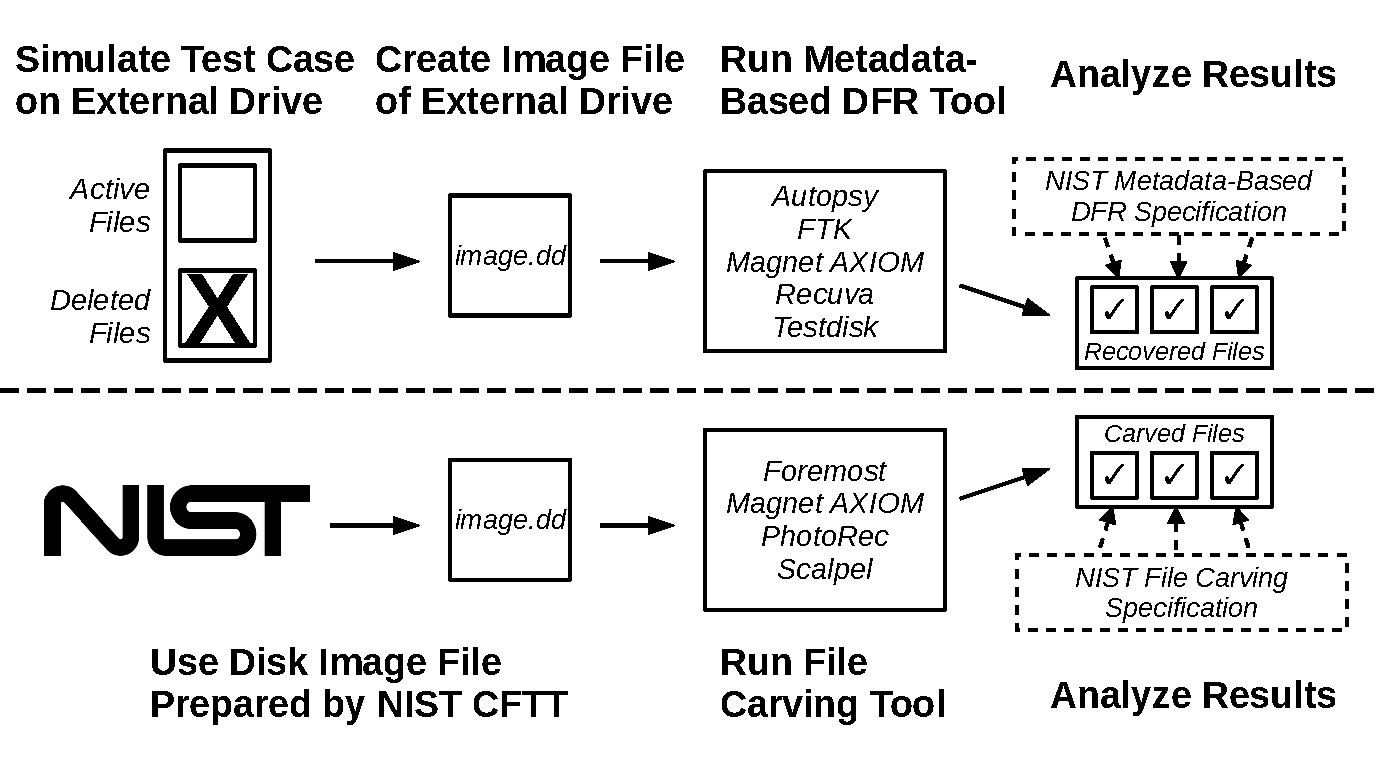
\includegraphics[width=\linewidth]{fig/overview.pdf}
    \caption{
        A read-only \emph{disk image}, a file which contains the raw data of a file system, is obtained for each test case.
        For metadata-based test cases, we create a file system on an external drive and delete files from it, then save it as a disk image.
        For file carving test cases, we use a set of disk images prepared by NIST CFTT.
        In either case disk image is input to a DFR tool, whose output is checked for compliance with the NIST guidelines for metadata-based DFR or file carving, depending on the tool.
    }
    \label{fig:overview}
\end{figure}

\subsection{Metadata-Based Tools}
\subsubsection{Designing Recovery Scenarios}

We begin by designing a set of test cases to simulate common challenges of metadata-based deleted file recovery.
In order to get the most information possible about each tools' capabilities, we design our test cases to be atomic.
We first isolate the most basic challenges of file recovery, and create test cases for them.
Then, we create test cases which combine those basic challenges.
Our intention with this atomic approach is to create test cases that are generalizeable to the majority of recovery scenarios, even the many which we do not explicitly cover.

In addition to this philosophy, we must remain within the scope of the NIST guidelines.
NIST requires test images to be ``created and deleted in a process similar to how an end-user would create and delete files.''~\cite{meta:dfr:standards}
We take this to mean that any interaction with the file system must be through a standard operating systems'  read and write operations.
We are not allowed to edit the file system directly, as ``files and file system metadata that is specifically corrupted, modified, or otherwise manipulated to appear deleted''~\cite{meta:dfr:standards} are explicitly out of scope.

Within these constraints, we can induce two phenomena which make file recovery more challenging: fragmentation and overwriting.
Following the aforementioned goal of making our tests atomic, all our test cases (besides the first trivial case) use fragmented and/or overwritten files as building blocks.
As such, our test cases fall into five general categories:
{\bf(a)} no fragmentation or overwriting, 
{\bf (b)} only fragmentation,
{\bf (c)} only overwriting,
{\bf (d)} both fragmentation and overwriting,
and {\bf (e)} fragmentation ``out of order.''


Each test case is listed in Table~\ref{meta_cases} along with a brief description.
We have given each a distinct name in line with the naming scheme for the CFTT file carving test cases.
A selection of test cases are illustrated, with each column portraying the state of the file system at a point in time. 
Each file is given a unique letter and shading, and the start and end of a fragmented file are denoted when relevant.

\begin{table}[ht!]
\tbl{Metadata-based DFR test cases}
{\begin{tabular*}{\textwidth}{@{}rp{0.8\linewidth}@{}} \toprule
\multicolumn{2}{c}{\textbf{Basic Deleted File}} \\ \colrule
\textbf{basic} & Deleted file is contiguous and the only file on the disk \\
\colrule
\multicolumn{2}{c}{\textbf{Deleted File is Fragmented}} \\ \colrule
\textbf{fragments1} & Deleted file is fragmented around an active file (illustrated in Figure~\ref{fig:case2}) \\
\textbf{fragments2} & Deleted file is fragmented around another deleted file \\
\colrule
\multicolumn{2}{c}{\textbf{Deleted File is Overwritten}} \\ \colrule
\textbf{overwrite1} & Deleted file is overwritten at the front by an active file \\
\textbf{overwrite2} & Deleted file is overwritten in the middle by an active file (illustrated in Figure~\ref{fig:case5}) \\
\textbf{overwrite3} & Deleted file is completely overwritten by an active file \\
\textbf{overwrite4} & Deleted file is overwritten at the front by another deleted file (illustrated in Figure~\ref{fig:case8}) \\
\textbf{overwrite5} & Deleted file is overwritten in the middle by another deleted file \\
\textbf{overwrite6} & Deleted file completely overwritten by another deleted file \\
\colrule
\multicolumn{2}{c}{\textbf{Deleted File is Fragmented and Overwritten}} \\ \colrule
\textbf{combo1} & Deleted file is fragmented around an active file, and the second fragment is overwritten by another active file (illustrated in Figure~\ref{fig:case12}) \\
\textbf{combo2} & Deleted file is fragmented around an active file, and the second fragment is overwritten by another deleted file \\
\colrule
\multicolumn{2}{c}{\textbf{Deleted File is Fragmented Out-of-Order}} \\ \colrule
\textbf{disorder1} & Deleted file fragmented out-of-order (illustrated in Figure~\ref{fig:case14}) \\
\textbf{disorder2} & Deleted file fragmented out-of-order with an active file in between the fragments \\
\textbf{disorder3} & Deleted file fragmented out-of-order with a deleted file in between the fragments \\
\botrule
\end{tabular*}}
\label{meta_cases}
\end{table}


\begin{figure}
    \centering
    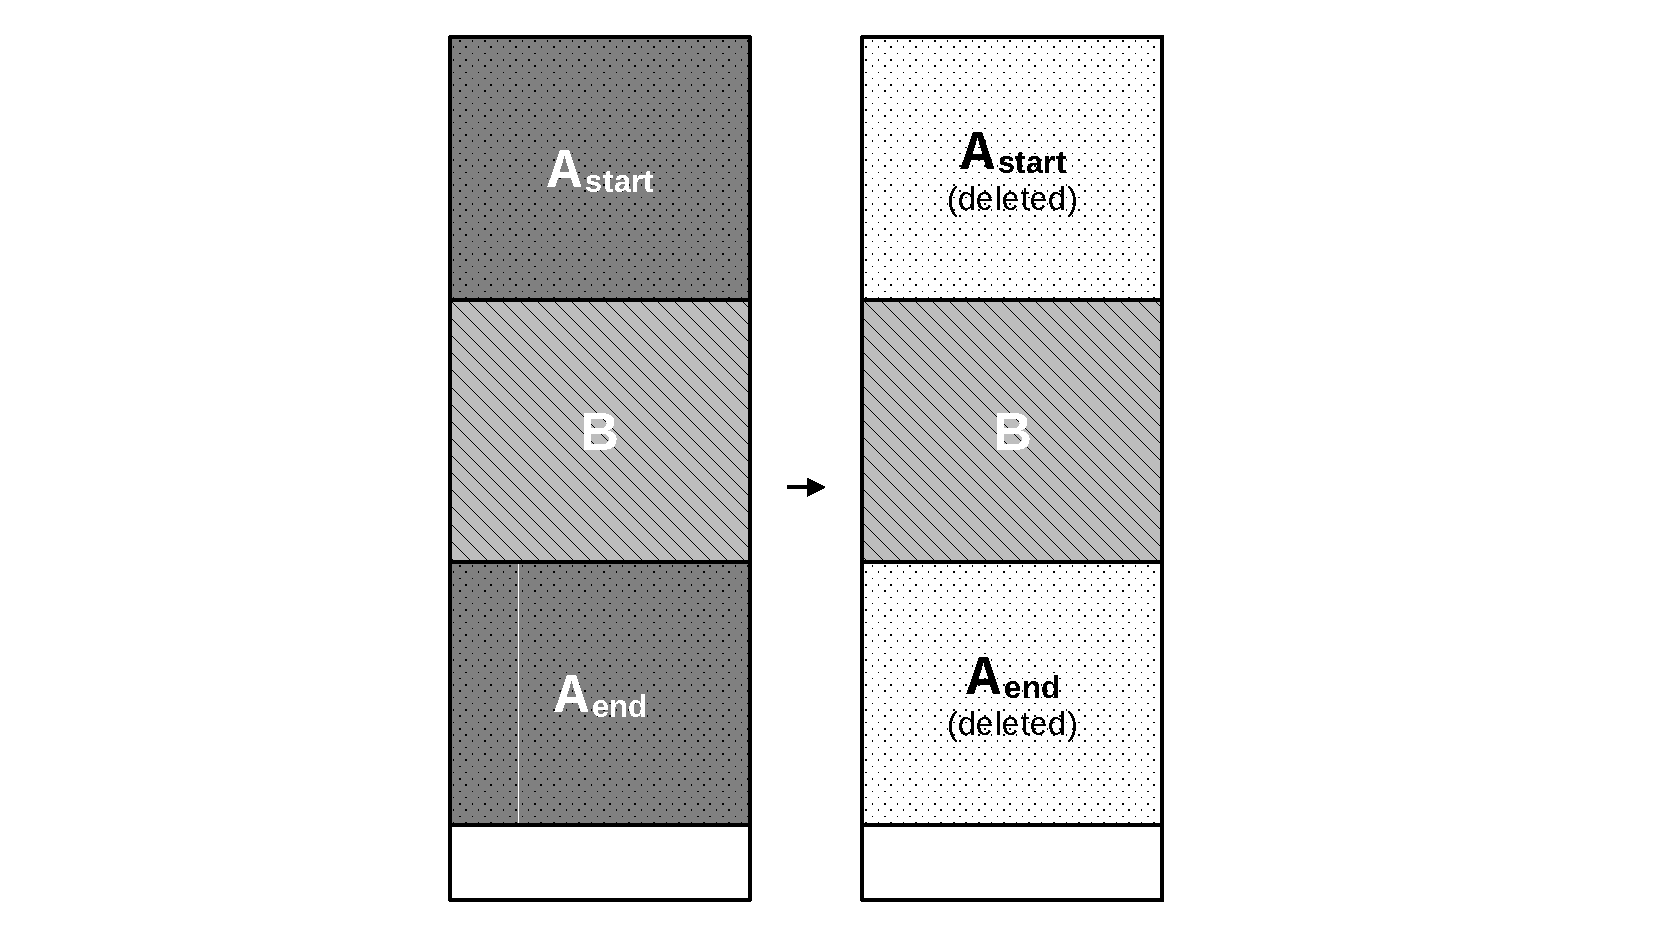
\includegraphics[width=\linewidth]{fig/case2.pdf}
    \caption{fragments1: File A is fragmented, and has been deleted.}
    \label{fig:case2}
\end{figure}

\begin{figure}
    \centering
    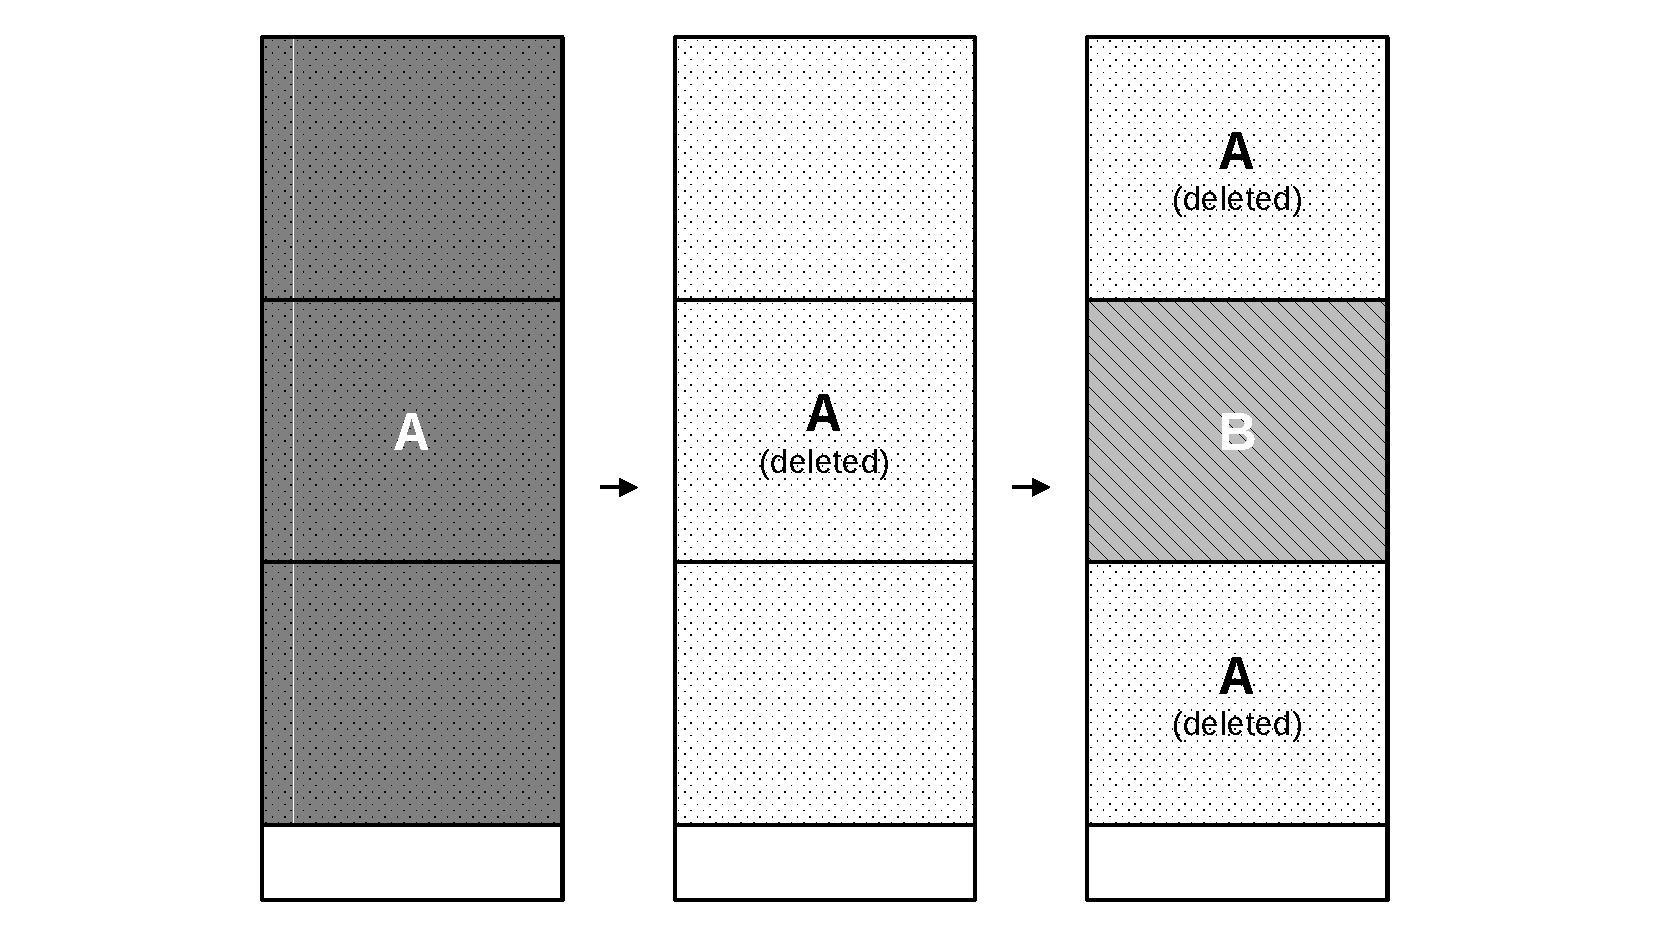
\includegraphics[width=\linewidth]{fig/case5.pdf}
    \caption{overwrite1: File A has been deleted and partially overwritten by file B.}
    \label{fig:case5}
\end{figure}

 \begin{figure}[h]
    \centering
    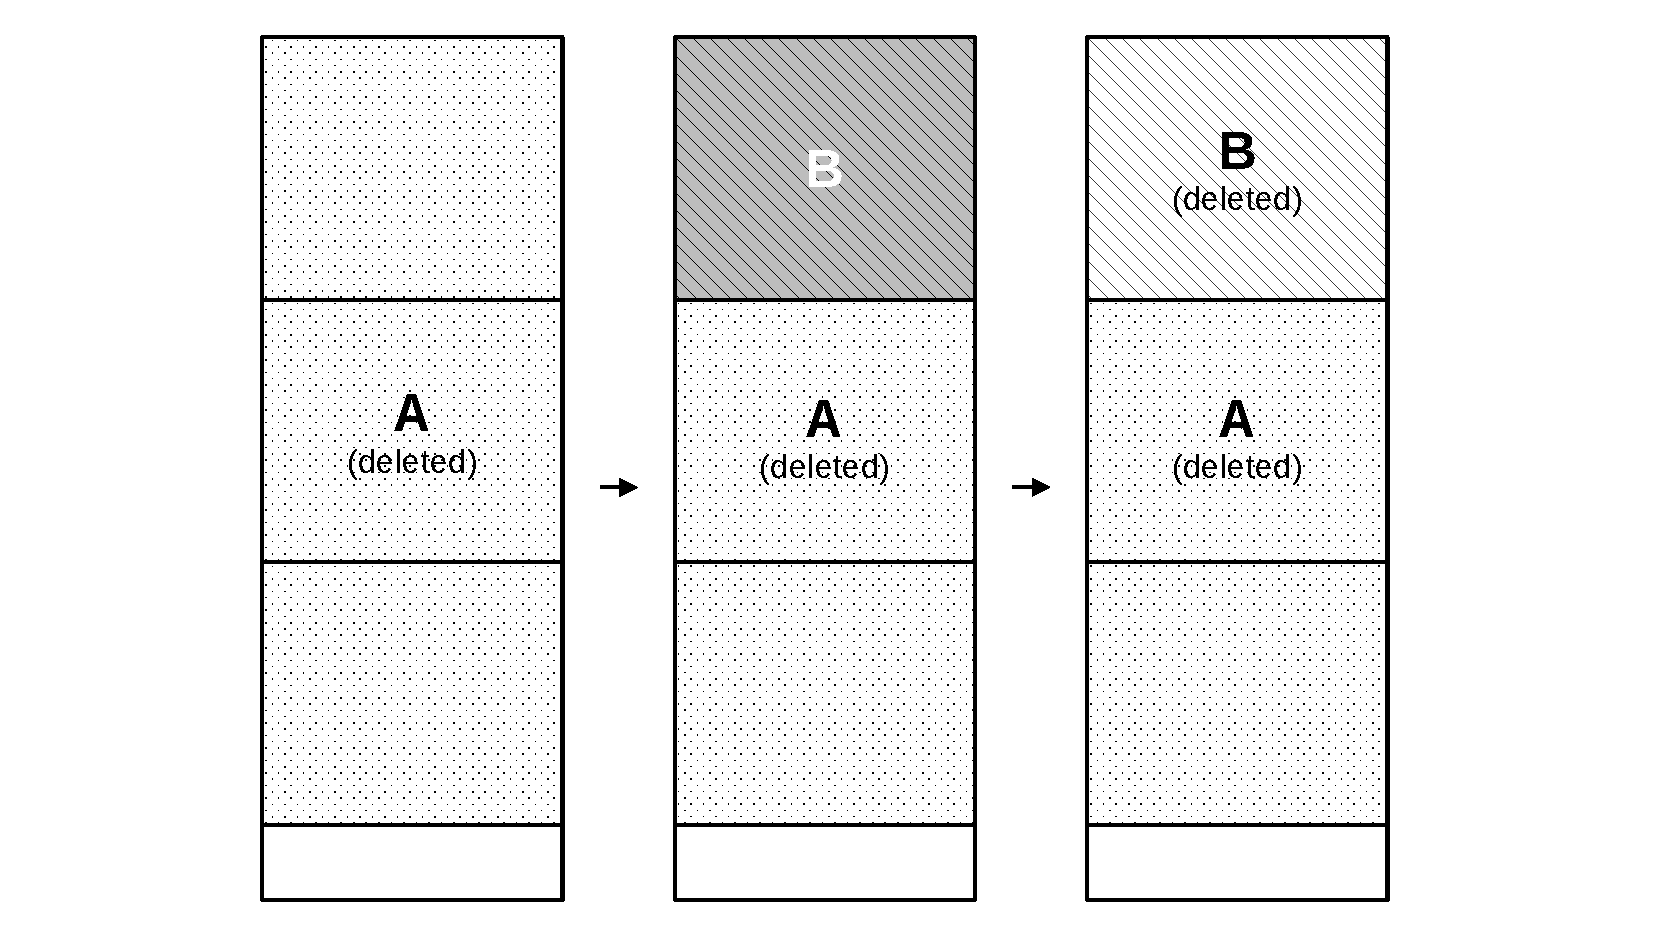
\includegraphics[width=\linewidth]{fig/case8.pdf}
    \caption{overwrite4: File A has been deleted and partially overwritten by file B, which has since been deleted}
    \label{fig:case8}
\end{figure}

\begin{figure}[h]
    \centering
    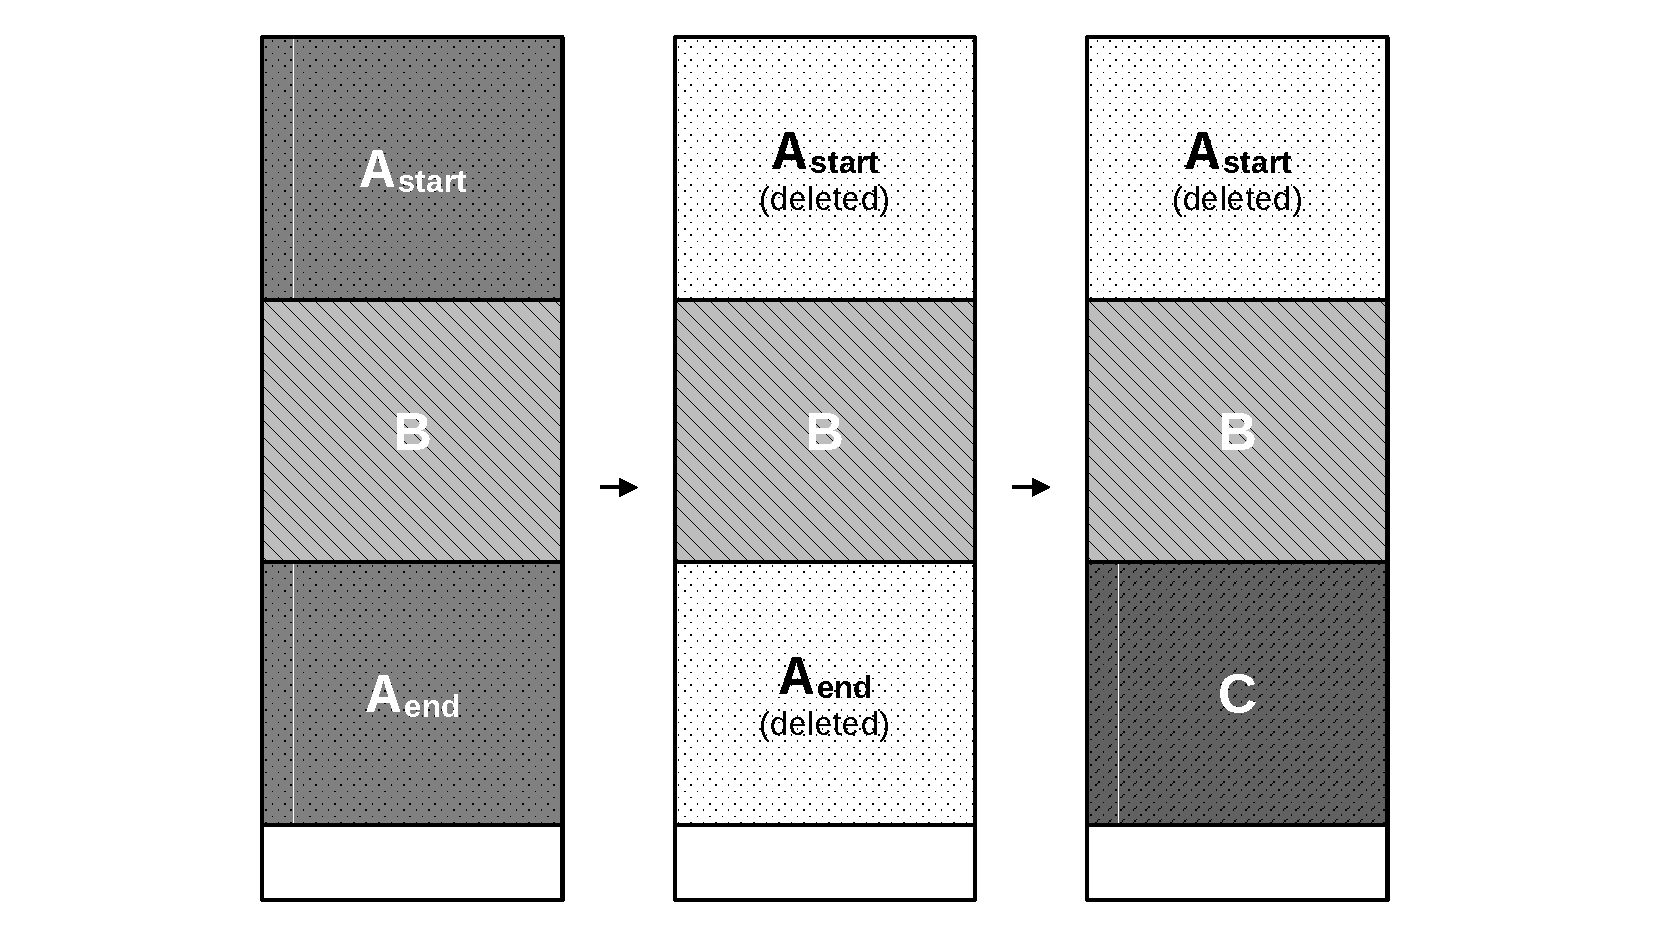
\includegraphics[width=\linewidth]{fig/case12.pdf}
    \caption{combo1: File A is fragmented and has been deleted. The second fragment has then been overwritten by file C}
    \label{fig:case12}
\end{figure}

\begin{figure}[h]
        \centering
        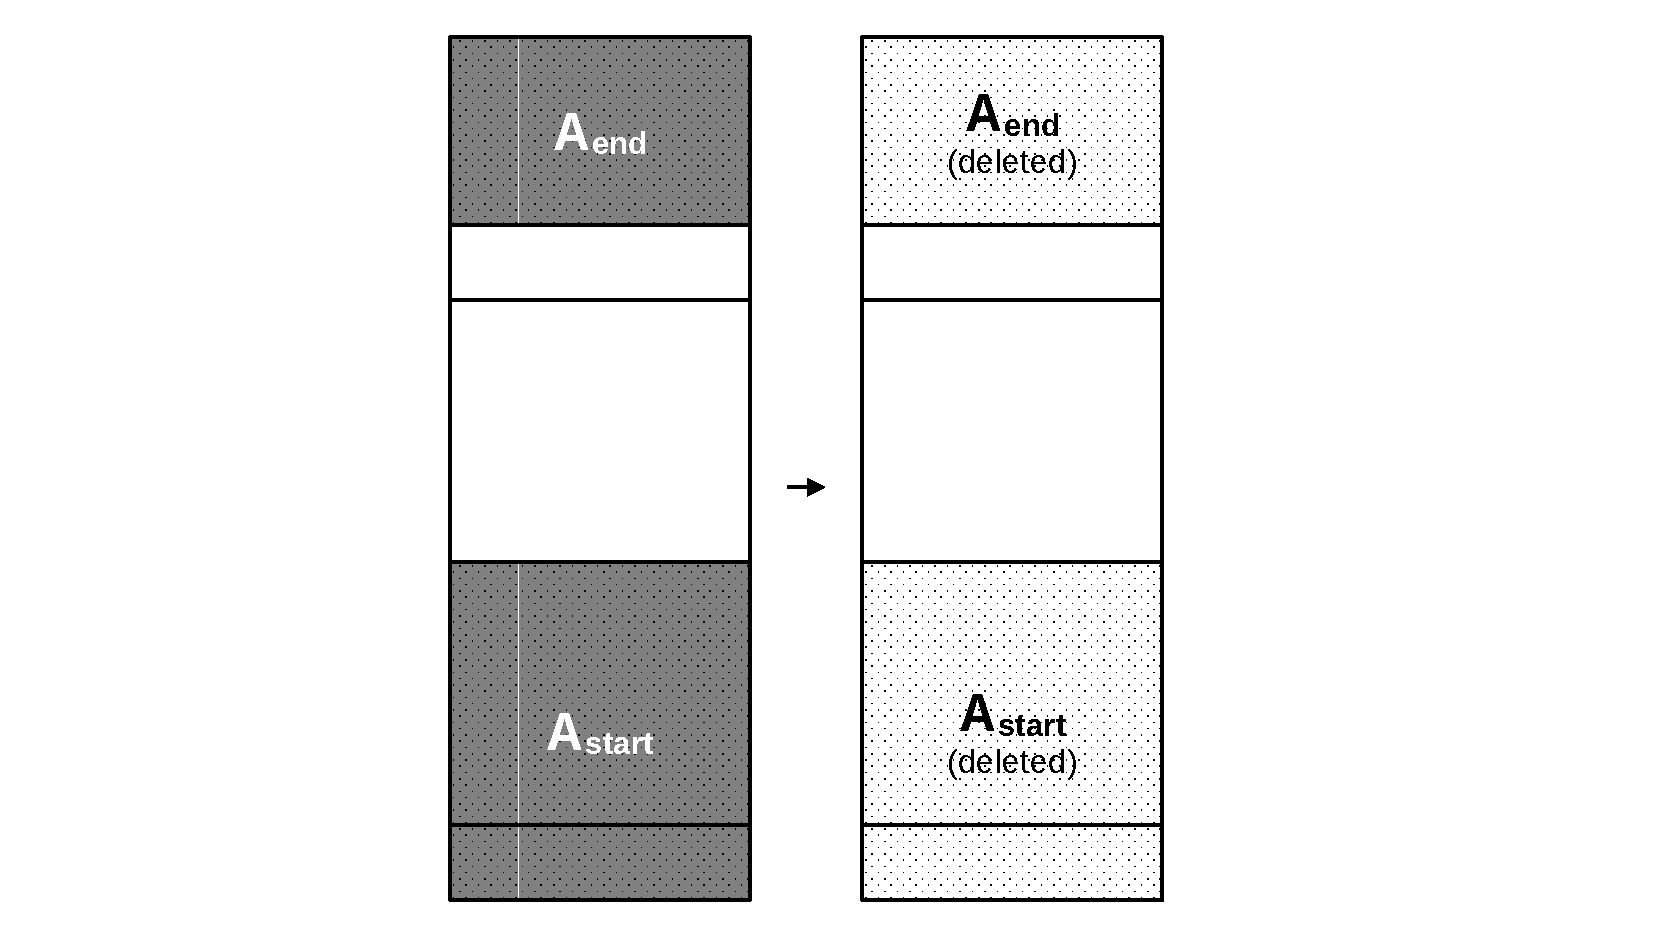
\includegraphics[width=\linewidth]{fig/case14.pdf}
        \caption{disorder1: File A is fragmented out-of-order, and has been deleted}
        \label{fig:case14}
\end{figure}


Fragmentation is trivial in NTFS because information about the runs of a file persist after deletion.
Since this renders the \emph{fragments} and \emph{disorder} cases functionally identical, we test only the \emph{fragments} cases for NTFS.
Cases \emph{overwrite2} and \emph{overwrite5} cannot be created through regular file operations in NTFS, due to NTFS's file allocation behavior.
Thus, we also exclude \emph{overwrite2} and \emph{overwrite5} for NTFS.
We do not exclude any test cases when using FAT.


\subsubsection{Creating Test Images}

We create the test cases on a 32 GB flash drive, using 4 MiB partitions for FAT cases and 6 MiB partitions for NTFS cases.
For each case, it is important to start by writing over the partition with zeroes, ensuring the image is easily reproducible.
Next, a file system should be written to the partition, and files should be written to it and deleted until the file system matches one of the planned test cases.
We used text files, each containing a single repeated letter (e.g., ``aa1M'' is a text file containing 1 MiB of the letter `a')
Note that text files cannot be recovered with file carving, so this choice forces tools which combine both DFR methods to rely solely on metadata-based recovery.
We write files to the test file system by copying them from another drive, and appending to files when we need to force fragmentation.
Once the test file system matches one of the planned test cases, we use the \emph{dd} utility to create a disk image of that partition.
Since the disk image can be made read-only, it is safer and more convenient to run tests on the disk image instead of the physical drive.
Note that we create FAT test cases using Ubuntu 18.04 and NTFS test cases using Windows 10.

\subsubsection{Challenges}

 % Caching problem
Creating test images can be difficult without a solid understanding of low-level file system behavior.
For example, a newly written file may not have its data written to the disk right away.
Even with fast modern storage, disk I/O involves a considerable amount of overhead.
To improve performance, operating systems generally prefer to write data in one larger batch versus several small batches.
So, the operating system will often store write operations in a cache and wait for a more optimal moment to actually write to the disk.
Typically, this optimization only causes problems in the event of sudden power loss or improper shutdown, but it can also make the state of the file system less predictable.
We found that we were often deleting a file while it was still cached, meaning it would never be written to the disk to begin with.
This is obviously a problem as it leaves nothing on the disk to recover.
Thankfully, Linux and Windows both provide a \emph{sync} system call, which causes the cached writes to be performed immediately.
Calling sync before each file deletion resolves the issue; alternatively, unmounting the file system triggers similar behavior.

% Learning and using the allocation algorithms
Since most of the test images involve manipulating file data into certain arrangements, it is also helpful to have some understanding of allocation algorithms.
Allocation algorithm refers to the steps the operating system takes to decide where on the disk to write new data.
Generally, the operating system wants to limit fragmentation, as contiguous files are more efficient to read and write to.
Common allocation algorithms like ``first available,'' ``next available,'' and ``best fit'' will place files according to that general principle, but use differing strategies to do so.
Understanding the allocation algorithm removes a lot of trial and error from the process of making test images.
For example, we observed that Linux uses a ``next available'' algorithm when writing to FAT.
After mounting the file system, the first file to be written will be placed at the first available space in the file system.
However, unlike the ``first available'' algorithm, the operating system remembers where it last placed a file, and it will place the next file at the first available space after that saved location, even if space opens up at the beginning of the file system.
Windows, on the other hand, uses a ``best fit'' algorithm when writing to NTFS.
This allocation algorithm takes a more proactive approach to reducing fragmentation by writing each file to the smallest space in which it can fit without being fragmented.


\subsubsection{Recovering Files}
\begin{paraphrase}
 We selected five popular DFR tools for testing: Autopsy~\cite{autopsy}, Recuva~\cite{recuva}, FTK Imager~\cite{ftk}, TestDisk~\cite{testdisk}, and Magnet AXIOM~\cite{axiom_meta}. 
Note that Autopsy uses a set of DF tools known as The Sleuth Kit (TSK) for metadata-based recovery, so TSK is also implicitly covered by this study. 
These tools were chosen based on popularity and availability.

The settings we used when testing each tool are as follows:
For Autopsy, we performed a standard recovery with all ingest modules disabled.
For Recuva we performed a standard recovery using the free version with default settings.
For FTK Imager, we performed a standard recovery using the free version with default settings.
For TestDisk we used the ``file undelete'' feature under ``Advanced Filesystem Utils.''
For Magnet AXIOM we performed a ``full scan'' in AXIOM Process and exported all files accessible in ``Filesystem View'' in AXIOM Examine.
\end{paraphrase}

\subsubsection{Results}

\begin{figure}
    \centering

    \begin{subfigure}[t]{0.3\linewidth}
        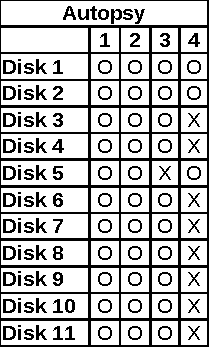
\includegraphics[width=\linewidth]{fig/autopsy_results_fat.pdf}
        \subcaption{Autopsy}
    \end{subfigure}~~
    \begin{subfigure}[t]{0.3\linewidth}
        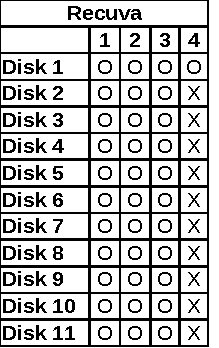
\includegraphics[width=\linewidth]{fig/recuva_results_fat.pdf}
        \subcaption{Recuva}
    \end{subfigure}
    \begin{subfigure}[b]{0.3\linewidth}
        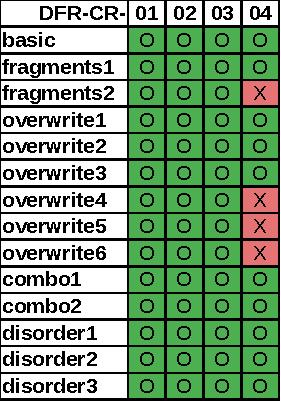
\includegraphics[width=\linewidth]{fig/ftk_results_fat.pdf}
        \subcaption{FTK}
    \end{subfigure}~~
    \begin{subfigure}[b]{0.3\linewidth}
        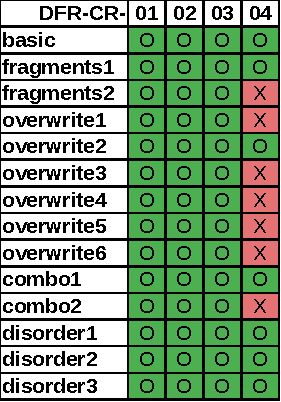
\includegraphics[width=\linewidth]{fig/testdisk_results_fat.pdf}
        \subcaption{TestDisk}
    \end{subfigure}~~
    \begin{subfigure}[b]{0.3\linewidth}
        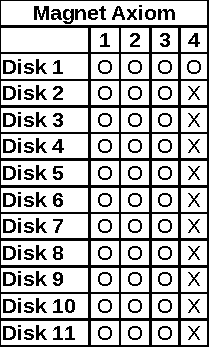
\includegraphics[width=\linewidth]{fig/axiom_results_fat.pdf}
        \subcaption{Magnet AXIOM}
    \end{subfigure}~~
        
    \caption{Test results on metadata-based DFR tools using FAT-formatted test images. Each row corresponds to a test image and each column corresponds to a core feature. An 'O' indicates success and an 'X' indicates failure.}
    \label{fig:results_fat}
\end{figure}

\begin{figure}
    \centering

    \begin{subfigure}{0.3\linewidth}
        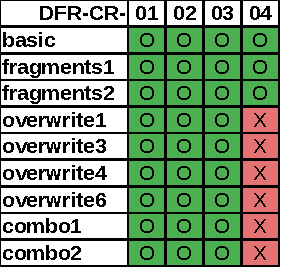
\includegraphics[width=\linewidth]{fig/autopsy_results_ntfs.pdf}
        \subcaption{Autopsy}
    \end{subfigure}~~
    \begin{subfigure}{0.3\linewidth}
        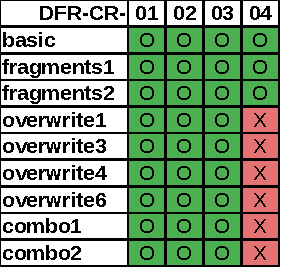
\includegraphics[width=\linewidth]{fig/recuva_results_ntfs.pdf}
        \subcaption{Recuva}
    \end{subfigure}
    \begin{subfigure}{0.3\linewidth}
        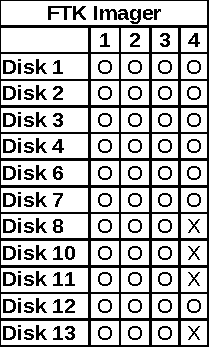
\includegraphics[width=\linewidth]{fig/ftk_results_ntfs.pdf}
        \subcaption{FTK}
    \end{subfigure}~~
    \begin{subfigure}{0.3\linewidth}
        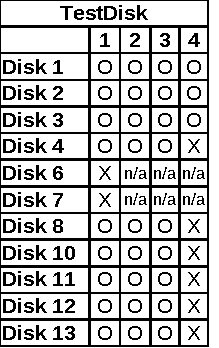
\includegraphics[width=\linewidth]{fig/testdisk_results_ntfs.pdf}
        \subcaption{TestDisk}
    \end{subfigure}~~
    \begin{subfigure}{0.3\linewidth}
        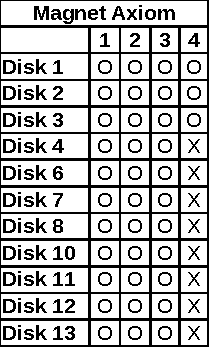
\includegraphics[width=\linewidth]{fig/axiom_results_ntfs.pdf}
        \subcaption{Magnet AXIOM}
    \end{subfigure}~~
        
    \caption{Test results on metadata-based DFR tools using NTFS-formatted test images. Each row corresponds to a test image and each column corresponds to a core feature. An 'O' indicates success and an 'X' indicates failure.}
    \label{fig:results_ntfs}
\end{figure}


After running a DFR tool for a test case, we examine the files output by the tool to see if the NIST guidelines have been met.
Note that a file does not need to be perfectly recovered for a tool to meet the guidelines, although all the guidelines would be met in that case.
Sometimes, as with overwritten files, part of the file's data literally no longer exists on the disk, so recovering the entire file is impossible.
The NIST guidelines are designed with this reality in mind.

Most tools recover files perfectly for FAT fragments1, and all tools recover files perfectly for FAT basic, NTFS basic, and NTFS fragments1 and fragments2.
For the other cases, we need to examine the recovered files closely to see which core features are being met.
We judge each tool as either meeting or failing each core feature individually for each test case.
Results are shown in Figure~\ref{fig:results_fat} and Figure~\ref{fig:results_ntfs} for FAT and NTFS test cases, respectively.

Note that in the one test case where DFR-CR-01 is not met, meaning no deleted file was detected, we cannot make a judgement for the other core features as they are all dependent on DFR-CR-01.



\paragraph{Recovering Fragmented Files}
We observe that tools typically use one of two strategies in the event of FAT fragmentation.
The first is to simply ignore fragmentation and recover the full length of a file as though it is contiguous, even if there are active files in that length.
Recuva and Magnet AXIOM seem to take this approach.
The second strategy is to still recover the full length of the file, but only from unallocated space.
So, any active files will be skipped over.
Autopsy, FTK, and TestDisk seem to take this approach.
This is most easily observed in FAT fragments1; Autopsy, FTK, and TestDisk will skip over file B to recover all of file A, while Recuva and Magnet AXIOM will recover the first fragment of file A along with the active file B.
This is why Recuva and Magnet AXIOM fail DFR-CR-04 for that case.
However, when a file is fragmented around another deleted file, like in FAT fragments2, all tools take the first approach and erroneously return file B as part of file A.
All tools seem to struggle with out-of-order fragmentation.
When the first fragment is at the very end of the file system, Recuva, FTK, and TestDisk only recover the first fragment, Autopsy returns a small amount of null data, and Magnet AXIOM returns an empty file and an error message.

In NTFS more information about a file's location remains after the file is deleted, so recovering fragmented files is trivial.
All tools we tested are able to handle fragmentation in NTFS with no issues.


\paragraph{Recovering Overwritten Files}
We observe that when a deleted file is overwritten by an active file, most tools still attempt to recover the overwritten part as though it was part of the original file, failing DFR-CR-04.
The only tool to consistently meet DFR-CR-04 in these cases is FTK Imager, which only recovers data from before the overwritten part.
TestDisk also does this for FAT overwrite2 only, otherwise behaving like the other tools.
In FAT, Autopsy only recovers the first cluster of an overwritten file, regardless of what part was overwritten.
In NTFS, it gives the same results as other tools.
For FAT overwrite1 and overwrite2, Magnet AXIOM recovers up to the end overwritten sections, but no further.
This is a bit strange as it suggests Magnet AXIOM can detect overwriting, but still returns the overwritten part.
For other cases it behaves like the other tools.

When a deleted file is overwritten by another deleted file, even FTK acts as though the overwritten part belongs to the original file.
This suggests that the tools which can detect overwriting do so based on the allocation status of each data block; other than that, they only consider the metadata of the file being recovered, not the files around it.

\paragraph{Miscellaneous}
Several FAT test cases (overwrite2, combo1, disorder1, disorder2, and disorder3) cause Autopsy to return a 1.5 KiB file containing null data.
This is particularly odd because a FAT cluster is 2 KiB; making these the only recovered objects not divisible into clusters.
Given the odd size and contents, we suspect this is some sort of error state rather than an attempted recovered file.

TestDisk does not identify any deleted file in NTFS overwrite3.
While the deleted file's data is entirely overwritten in this case, information about the file is still present in metadata.
Since this only happens in NTFS and not FAT, meaning the precise location of the deleted file is still available, it is possible that TestDisk is able to detect the fact that the file has been overwritten, and simply ignores it.
Even if this is the case, the file information is still available in metadata, so the for TestDisk to meet DFR-CR-01, it must identify the file regardless of whether it can be recovered.


\subsection{Carving-Based Tools}

\subsubsection{CFTT Test Cases}
To evaluate the file carving tools, we used six disk images prepared by CFTT\cite{cftt_carving_images}.
Each of these images contains between 20 and 40 graphical files of the JPG, PNG, GIF, BMP, and TIFF formats.
Importantly, the CFTT images do not contain valid file systems.
This ensures that a tool which utilizes both DFR methods can be evaluated solely on its file carving ability.

Despite the differences between the methods, metadata-based DFR and file carving are complicated by the same two file-system behaviors: fragmentation and overwriting. Thus, the CFTT test cases are somewhat similar to the ones we created for metadata-based DFR; each is built around a specific variation of fragmentation or overwriting of deleted files.
Following are summaries of each CFTT test image:
\begin{itemize}
 \item \textbf{basic:} 40 contiguous files, with space in between each file
 \item \textbf{nofill:} 40 contiguous files, with no space in between each file
 \item \textbf{simple-frag:} 40 fragmented files, with space in between each fragment
 \item \textbf{braid:} 10 contiguous files and 10 fragmented files, which are fragmented around each other in an A-B-A-B pattern
 \item \textbf{disorder:} 35 fragmented files, 30 of which are fragmented out-of-order such that the fragment containing the footer comes before the fragment containing the header
 \item \textbf{partials:} 15 complete files, 5 of which are fragmented, and 25 incomplete files where at least one fragment has been overwritten or manually destroyed

\end{itemize}


\subsubsection{Recovering Files}

We selected four popular file carving tools for testing: PhotoRec~\cite{photorec}, Foremost~\cite{foremost}, Scalpel~\cite{scalpel}, and Magnet AXIOM~\cite{axiom_carve}.
Note that since tests were run at different times, the version of Magnet AXIOM used for carving tests is newer than the version used for metadata-based tests.

The settings we used when testing each tool are as follows:
For PhotoRec and Foremost, we used the default settings.
For Scalpel, we manually enabled recovery of the JPG, PNG, GIF, BMP, and TIFF formats, and otherwise used default settings.
For Magnet Axiom, we ran a ``sector-level scan'' with default settings in AXIOM Process and exported all graphical files from ``Artifact View'' in AXIOM Examine.
We also exported an XML carving report from Axiom Examine as unlike the other tools it does not create one automatically.

\subsubsection{Evaluating Results}
The main challenge when testing file carving tools is verifying the results. 
For metadata-based tools this is fairly simple; the deleted files in our tests are all simple text files which can be checked at a glance.
However, text files lack a standard header and footer and thus cannot be recovered with file carving, so the test images use more complicated formats such as JPG.
As a result, it would be impractical to evaluate a tool based on the carved files alone.

Fortunately, all four of the carving tools we evaluated produce an itemized report of carving results. CFTT provides detailed information about the contents of the test images, so we can compare the tools' reports with the true arrangement of files in each image. This is particularly important for FC-CR-01, FC-CR-02, and FC-CR-03 since they are concerned with the specific data blocks the tool carves. PhotoRec's report gives a start and end address for each file, and multiple start and end addresses if it attempts to carve a fragmented file. The other tools' reports only list the starting address and size of each file, so we assumed they never attempt to carve more than one fragment per file.

Checking FC-CR-04 is slightly complicated by the fact that carving tools cannot recover the filename, but we can use the first sector listed for each file in the carving report to match them with the original files and check the file extensions.

For FC-CR-05, we make use of the \emph{identify} command from the ImageMagick~\cite{imagemagick} tool suite. Upon input of a graphical file, identify will output the file format and other information. Relevant to FC-CR-05 is that the return code will indicate whether the file is valid or corrupt. We add the \emph{-regard-warnings} flag so an error or warning while parsing the file will mean the file is considered corrupt.

\subsubsection{Results}

\begin{figure}
    \centering

    \begin{subfigure}{\linewidth}
        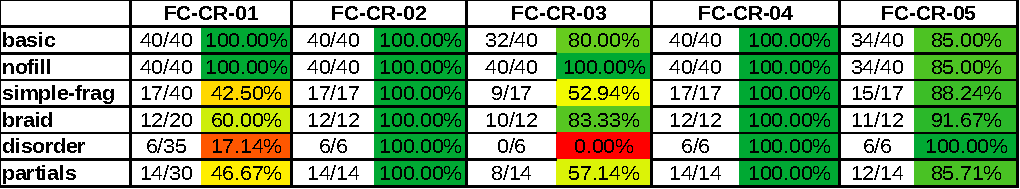
\includegraphics[width=\linewidth]{fig/photorec_results_carve.pdf}
        \subcaption{PhotoRec}
    \end{subfigure}
    \begin{subfigure}{\linewidth}
        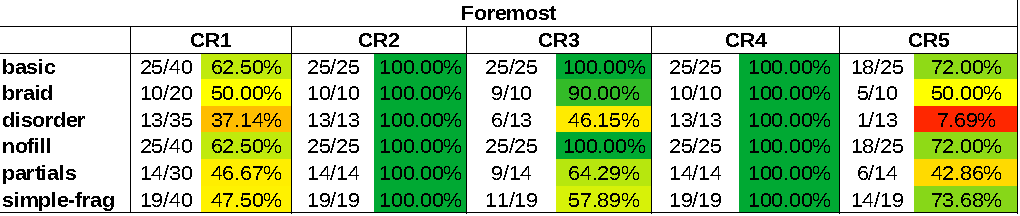
\includegraphics[width=\linewidth]{fig/foremost_results_carve.pdf}
        \subcaption{Foremost}
    \end{subfigure}
    \begin{subfigure}{\linewidth}
        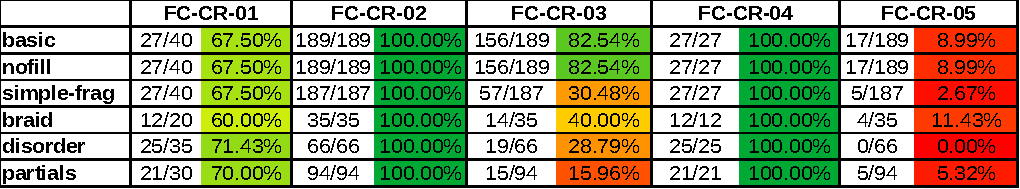
\includegraphics[width=\linewidth]{fig/scalpel_results_carve.pdf}
        \subcaption{Scalpel}
    \end{subfigure}
    \begin{subfigure}{\linewidth}
        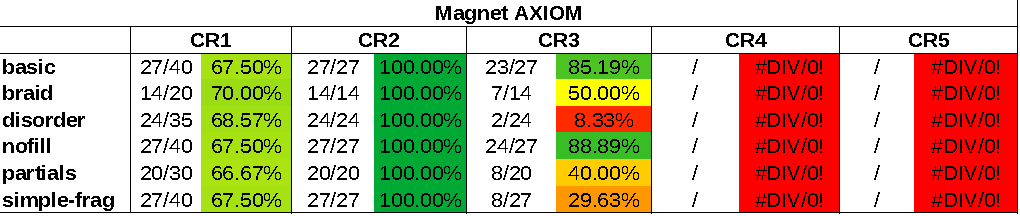
\includegraphics[width=\linewidth]{fig/axiom_results_carve.pdf}
        \subcaption{Magnet AXIOM}
    \end{subfigure}
        
    \caption{
    Results from testing file carving tools. 
    Each row represents a test case, and each column represents a core feature. 
    Since each test image contains many files, we score a tool's compliance with the NIST guidelines by determining the percentage of files for which each core feature is met.
    In each case, scores are given in both fractional and percent form.
    %For details on how the numbers are determined, see the explanation of core features in Section~\ref{sec:carving_features}.
    }
    \label{fig:results_carve}
\end{figure}

% CR1: hit rate, hits/source files
% CR2: in-bounds/carved, trivial
% CR3: one-source/carved, often still a valid file
% CR4: hits identified correctly/hits, trivial
% CR5: valid/carved, 

%Results for file carving tools can be seen in Figure~\ref{fig:results_carve}.

For FC-CR-01, Scalpel and Magnet AXIOM score between 60\% and 70\% for all test cases, Foremost scores between 37\% and 63\%, and PhotoRec ranges from a perfect score to as low as 17\% depending on the test case.
A high score on this core feature means a tool detects most of the original deleted files in a given test case, in other words, it has a high ``hit rate.''

All tools perfectly fulfil FC-CR-02, meaning they never try to carve data from outside the drive or partition given as input.

For FC-CR-03, each tool achieves high scores on some test cases and low score on others.
A high score on this core feature means most of the files a tool recovers contain data from only one other source.
Note that carving from multiple sources may still result in a valid file, such as in Figure~\ref{fig:CR3_fail}.

\begin{figure}
    \centering
    \begin{subfigure}{0.45\linewidth}
        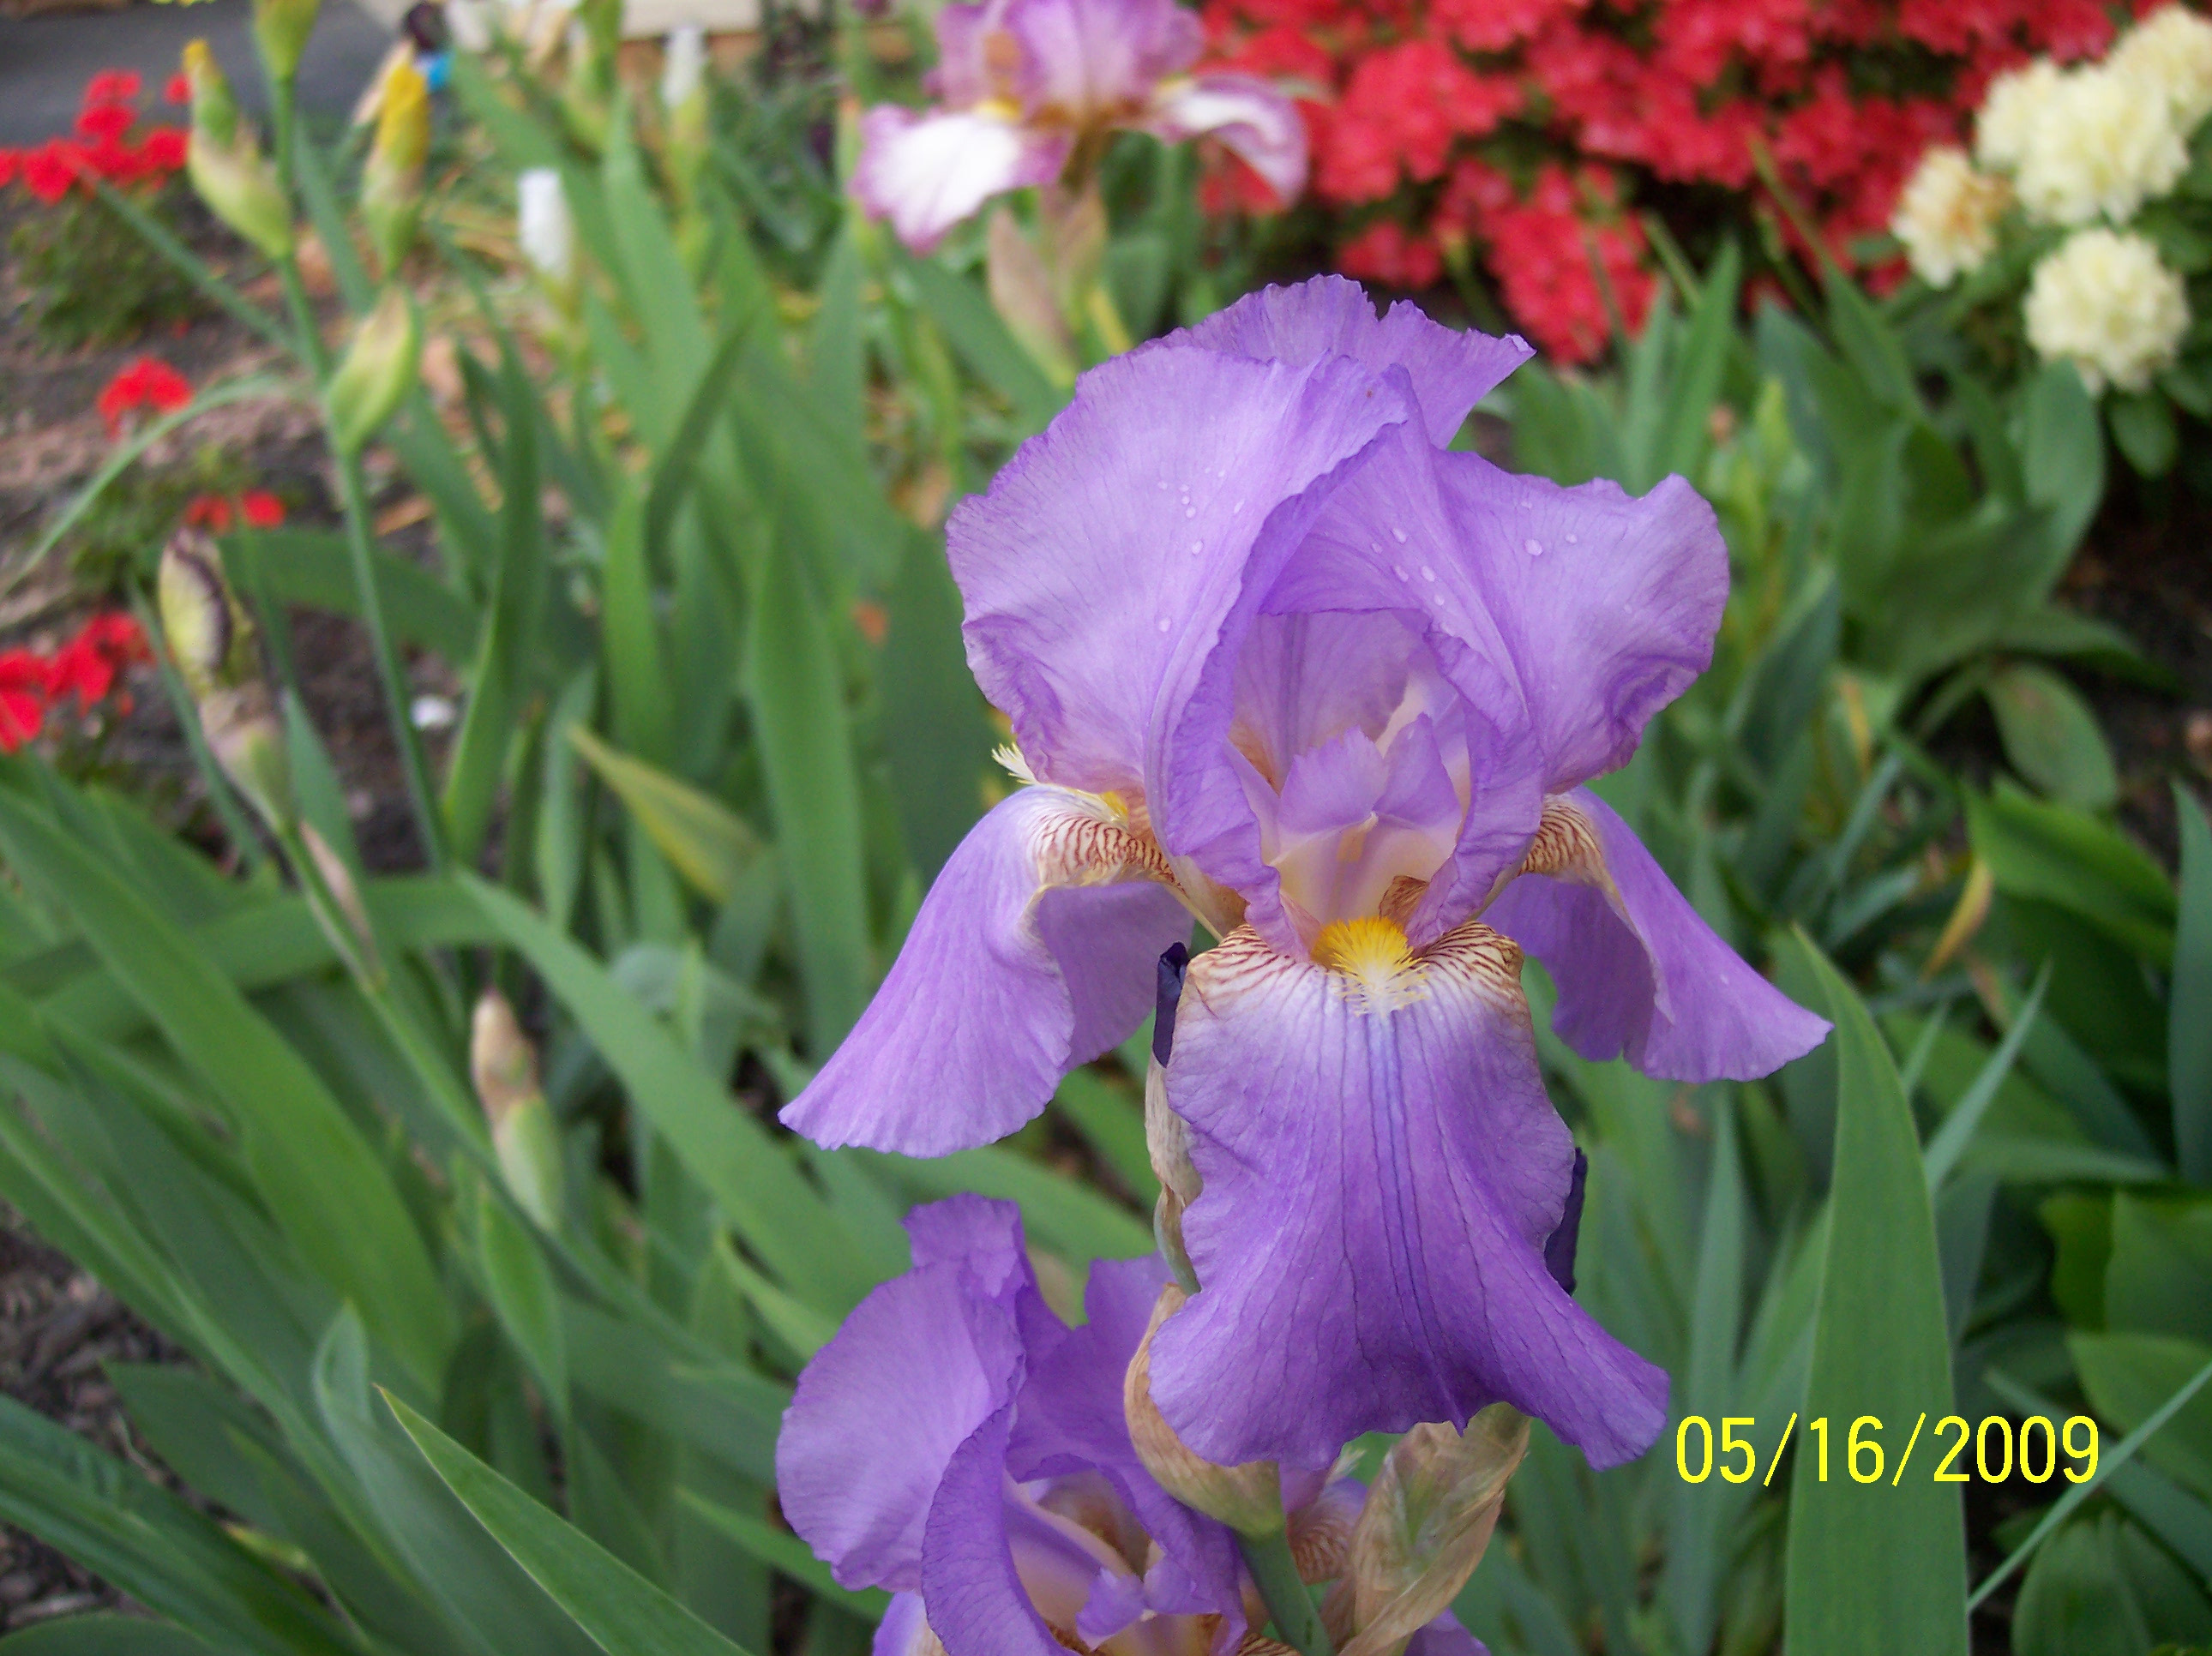
\includegraphics[width=\linewidth]{fig/iris-lavender.jpg}
        \subcaption{Original}
    \end{subfigure}
    \begin{subfigure}{0.45\linewidth}
        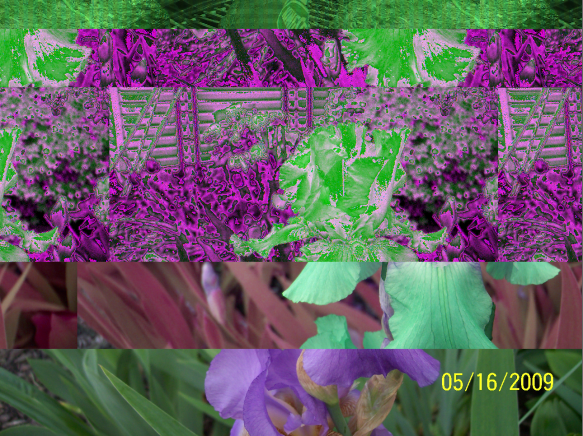
\includegraphics[width=\linewidth]{fig/CR3_fail.png}
        \subcaption{Carved}
    \end{subfigure}
    \caption{
        \emph{iris-lavender.bmp} from the \emph{disorder} test case, as carved by PhotoRec.
        By cross-referencing NIST CFTT's map of the test image with PhotoRec's report file, we find  that the carved file is actually composed of data from 3 files: \emph{iris-lavender.bmp}, \emph{iris-yellow.bmp}, and \emph{smoked-chicken.bmp}.
        In this case, PhotoRec fails to meet CF-CF-03, despite outputting a valid BMP image.
        }
    \label{fig:CR3_fail}
\end{figure}

All tools perfectly fulfil CF-CR-04, meaning every carved file that represents a ``hit,'' is given the same file extension as its corresponding original file.
We limit this only to ``hits,'' excluding false positives, to avoid overlapping with CF-CR-05.

For CF-CR-05, PhotoRec generally scores very high, Foremost and Magnet AXIOM get high scores for some test cases and low scores for others, and Scalpel scores very low for all test cases.
A high score on this core feature means most of the files a tool carves are valid files of some image format and can be properly parsed as that format (we test with the \emph{identify} tool from ImageMagick).
This may imply the tool checks carved files for validity before outputting them.
Note that identify throws a warning for six of the TIFF files used to create CFTT's test images, so we ignore the warning for carved versions of those six files.
